%; whizzy paragraph
%; whizzy-paragraph "^\\\\dancersection"
% -initex iniptex -latex platex -format platex -bibtex jbibtex -fmt fmt
% 以上 whizzytex を使用する場合の設定。

%     Tokyo Debian Meeting resources
%     Kansai Debian Meeting resources
%     Copyright (C) 2008 Junichi Uekawa
%     Copyright (C) 2008 Nobuhiro Iwamatsu

%     This program is free software; you can redistribute it and/or modify
%     it under the terms of the GNU General Public License as published by
%     the Free Software Foundation; either version 2 of the License, or
%     (at your option) any later version.

%     This program is distributed in the hope that it will be useful,
%     but WITHOUT ANY WARRANTY; without even the implied warranty of
%     MERCHANTABILITY or FITNESS FOR A PARTICULAR PURPOSE.  See the
%     GNU General Public License for more details.

%     You should have received a copy of the GNU General Public License
%     along with this program; if not, write to the Free Software
%     Foundation, Inc., 51 Franklin St, Fifth Floor, Boston, MA  02110-1301 USA

%   Pdf作成手順
% dvipdfmx debianmeetingresume2011-fuyu.dvi
%  preview (shell-command (concat "evince " (replace-regexp-in-string "tex$" "pdf"(buffer-file-name)) "&"))
% 画像ファイルを処理するためにはebbを利用してboundingboxを作成。
%(shell-command "cd image2012-fuyu; ebb *.png")


% progress memo:
% 2021/12 - 2022/11? がマージ対象
% イベント等でない場合は理由を書くこと。
% 必要な変更点は FIXME で記録しています。

%%ここからヘッダ開始。

\documentclass[mingoth,a4paper]{jsarticle}
\usepackage{monthlyreport}
\usepackage[dvips]{xy} % for advi workaround. Bug #452044
\usepackage{ulem}
\usepackage{wrapfig}
%\usepackage{pygmentize}

% コードハイライトの為の設定 for 201706 tokyo
\makeatletter\chardef\pdf@shellescape=\@ne\makeatother
\usepackage{minted}

% ページ調整のため部分的に2段組に
\usepackage{multicol}

\begin{document}

\begin{titlepage}
\thispagestyle{empty}

\hspace*{-2.5cm}
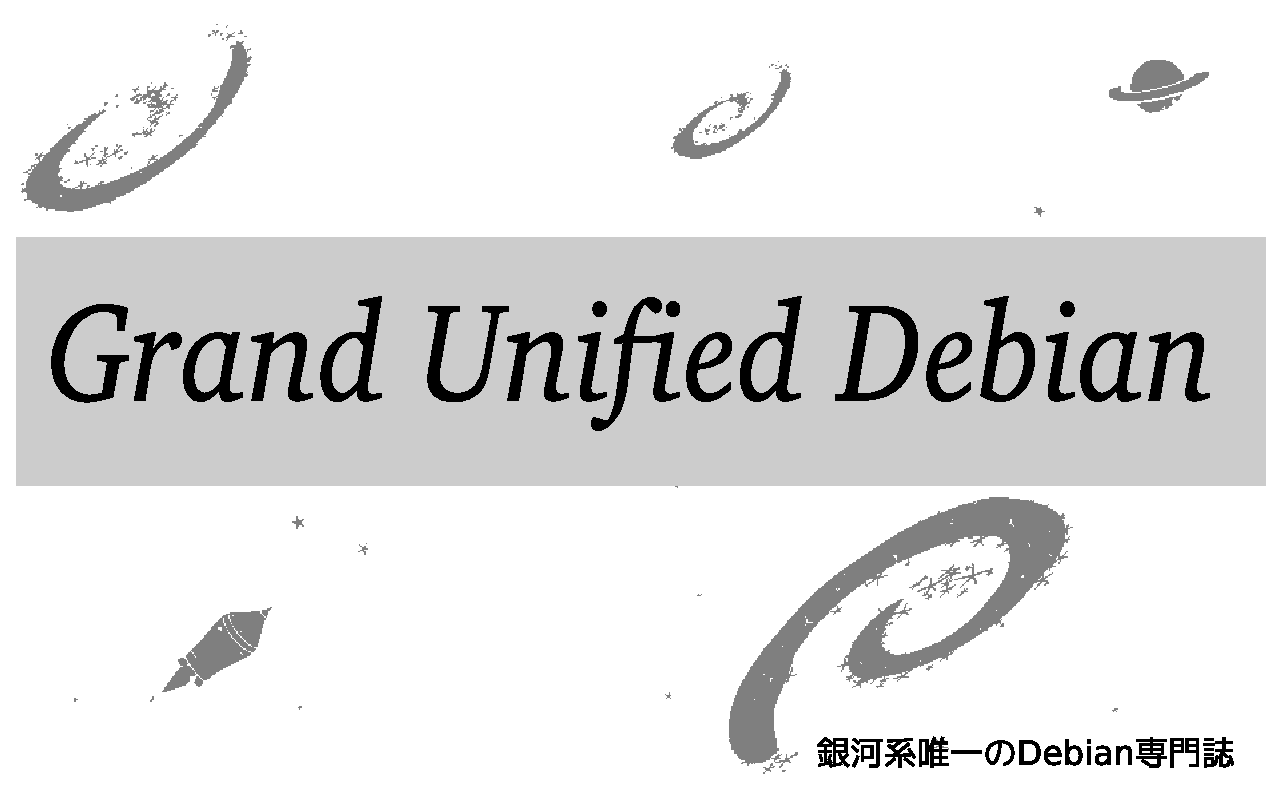
\includegraphics{../2012/image2012-natsu/gudeb.eps}\\
\\
\\
\rotatebox{10}{\fontsize{32}{32} {\gt 東京エリア/関西Debian勉強会}}

%\vspace*{-1.5cm}
\hspace*{11cm}\includegraphics[height=6cm]{../2005/image200502/openlogo-nd.eps}\\
\vspace*{0.1cm}
\hfill あんどきゅめんてっど でびあん 2022年冬号 2022年12月31日 初版発行
\end{titlepage}

\newpage
\thispagestyle{empty}\mbox{}
\newpage

% section の代わりの環境 -- 改訂する。
\renewcommand{\dancersection}[2]{%
\newpage
あんどきゅめんてっど でびあん 2022年冬号
%
% top line
\vspace{0.1mm}\\
{\color{dancerlightblue}\rule{\hsize}{2mm}}

%
% middle text
%
\begin{minipage}[t]{0.6\hsize}
\color{dancerdarkblue}
\vspace{1cm}
\section{#1}
\hfill{}#2\\
\end{minipage}
\begin{minipage}[t]{0.4\hsize}
\vspace{-2cm}
\hfill{}\includegraphics[height=8cm]{../2005/image200502/openlogo-nd.eps}\\
\vspace{-5cm}
\end{minipage}
%
%
{\color{dancerdarkblue}\rule{0.74\hsize}{2mm}}
%
\vspace{2cm}
}

\setcounter{page}{1}
\begin{minipage}[]{0.2\hsize}
 \definecolor{titleback}{gray}{0.9}
 \colorbox{dancerlightblue}{\rotatebox{90}{\fontsize{80}{80}
{\gt \color{dancerdarkblue}デビアン勉強会} }}
\end{minipage}
\begin{minipage}[]{0.8\hsize}
\hrule
\vspace{1mm}
\hrule
\setcounter{tocdepth}{1}
{\small
 \tableofcontents}
\vspace{1mm}
\hrule
\vspace{3cm}

\end{minipage}

% FIXME: 本文を追加すること。
%-------------------------------------------------------------------------------
\dancersection{Introduction}{DebianJP}
%-------------------------------------------------------------------------------

\subsection{東京エリアDebian勉強会}

 Debian勉強会へようこそ。これからDebianの世界にあしを踏み入れると
 いう方も、すでにどっぷりとつかっているという方も、月に一回Debianについ
 て語りませんか?

 Debian勉強会の目的は下記です。

\begin{itemize}
 \item \underline{Debian Developer} (開発者)の育成。
 \item 日本語での ``\underline{開発に関する情報}'' を整理してまとめ、アップデートする。
 \item \underline{場}の提供。
 \begin{itemize}
  \item 普段ばらばらな場所にいる人々が face-to-face で出会える場を提供
    する。
  \item Debian のためになることを語る場を提供する。
  \item Debianについて語る場を提供する。
 \end{itemize}
\end{itemize}

 Debianの勉強会ということで究極的には参加者全員がDebian Packageをがりがり
 と作るスーパーハッカーになった姿を妄想しています。情報の共有・活用を通し
 て Debianの今後の能動的な展開への土台として、 ``場'' としての空間を提供す
 るのが目的です。

\subsection{関西 Debian 勉強会}

 関西 Debian 勉強会はDebian GNU/Linux のさまざ
 まなトピック(新しいパッケージ、Debian 特有の機能の仕組、Debian 界隈で起
 こった出来事、などなど)について話し合う会です。

 目的として次の三つを考えています。
 \begin{itemize}
  \item MLや掲示板ではなく、直接顔を合わせる事での情報交換の促進
  \item 定期的に集まれる場所
  \item 資料の作成
 \end{itemize}

 それでは、楽しい一時をお楽しみ下さい。
 
%収録予定
%202112
%-------------------------------------------------------------------------------
\dancersection{Debian で Android アプリ開発と Kotlin}{杉本 典充}
%-------------------------------------------------------------------------------

\subsection{はじめに}

最近 Android アプリを開発しており、Debian で Android アプリを開発するには
どのような準備をすればよいのか、最近の Android アプリの開発で使われるプログラム言語「Kotlin」の Debian における対応状況について調べてみました。


\subsection{Debian で Android アプリを開発する}

\subsubsection{Android 情報のドキュメントの場所}

Android アプリの開発者向けのドキュメントは \url{https://developer.android.com/?hl=ja} にあります。

この Web ページでは Android アプリの開発に利用する Android Studio のダウンロードとインストール方法、最近の Android 情報や開発者ガイド、ガイドライン、チュートリアルなどの情報を公開しています。


\subsubsection{Android Studio のインストール}

Linux 環境に Android Studio をインストールする手順は、開発者向けドキュメントの \url{https://developer.android.com/studio/install?hl=ja#linux} に記載があり、Debian Wiki\footnote{\url{https://wiki.debian.org/AndroidStudio}} にも情報があります。インストール手順には tarball をダウンロードして任意のディレクトリに展開する方法と、snap 環境にインストールする方法があります。

ここでは、\url{https://developer.android.com/studio#downloads} から利用規約を読み承諾してダウンロードし\footnote{ダウンロードする tarball は 935 MiB ありますので、定額で高速にインターネット接続できる環境でセットアップすることをおすすめします。}、展開して Android Studio を起動するコマンドを示します。

\begin{commandline}
$ tar xf android-studio-2020.3.1.26-linux.tar.gz
$ cd android-studio/bin
$ bash studio.sh
\end{commandline}

studio.sh を起動すると、Android Studio の画面が表示され、実行に必要な追加のソフトウェアを大量にダウンロードします。ダウンロードとインストールが完了すると Android Studio を起動できます。

なお、Android Studio は IntelliJ IDEA ベースで作られています。そのため Android Studio を実行するには Java 環境が必要であり tarball の中に OpenJDK 11 が含まれています(Debian が提供する openjdk-11-jre パッケージをインストールせずに実行できます)。


\subsubsection{Android エミュレータを実行するために KVM を設定する}

Android アプリをデバッグするために Android のエミュレータ (=仮想マシン) が提供されています。Android のエミュレータのイメージファイルは qemu で動作する仮想マシンになっているため、PC 上で KVM を使えるように以下のパッケージをインストールします。

\begin{commandline}
# apt-get update
# apt-get install qemu-kvm
\end{commandline}


\subsubsection{Android アプリを実機でデバッグ実行できるように設定する}

Android Studio ではビルドした Android アプリをデバッグ実行することができます。デバッグ実行すると、設定したエミュレータ上または Android スマートフォンの実機上でアプリを動かすことができます。Android アプリを Android スマートフォンの実機上で実行する手順は、\url{https://developer.android.com/studio/run/device?hl=ja} に説明があります。

Debian では PC と Android スマートフォンの実機を USB 接続したことを検知するためのパッケージを提供しており、android-sdk-platform-tools-common パッケージをインストールすると udev の設定ファイルである "/lib/udev/rules.d/51-android.rules" をインストールします。パッケージのインストール後は、udev の設定ファイルを再読み込みします。なお、USB 接続する Android スマートフォンが Pixel シリーズの場合は、Debian 11 bullseye が提供する linux kernel にドライバが含まれているため、別途ドライバのインストールは不要です。

\begin{commandline}
# apt-get install android-sdk-platform-tools-common
# systemctl reload udev
\end{commandline}

次に Android スマートフォンを設定します。Android スマートフォンの設定画面を開いて開発者向けオプションを有効にし\footnote{「ビルド番号」の項目を7回連続でタップすると開発者向けオプションが有効になります。 \url{https://developer.android.com/studio/debug/dev-options?hl=ja}}、開発者向けオプションの設定画面にある「USB デバッグ」を有効にします。この状態の Android スマートフォンを Android Studio を実行している PC に USB 接続すると、Android スマートフォンの画面にフィンガープリントを確認する画面が出てきますので「はい」を選択します。少し待つと Android Studio の上部にある Android アプリの実行対象デバイスを表示するメニューに Android スマートフォン実機の型番が表示されます。ここまで準備ができると Android Studio でアプリをデバッグ実行すれば 実機で Android アプリを動かすことができます。


\subsection{Debian での Kotlin}

\subsubsection{ドキュメントの情報}

Kotlin の upstream の Web サイトは \url{https://kotlinlang.org/} にあり、ソースコードは Apache License 2.0 の下でソースコードを公開しています\footnote{\url{https://github.com/JetBrains/kotlin}}。2021 年 12 月 18 日現在では、バージョン 1.6.10 を提供しています。

Debian における Kotlin の情報は、\url{https://wiki.debian.org/Kotlin} に記載があります。Debian パッケージでは unstable のみですが  kotlin パッケージを提供しており(kotlin-1.3.31)、\url{https://salsa.debian.org/java-team/kotlin} で開発作業を進めています。upstream のバージョンと比べると Debian パッケージのものはだいぶ遅れている状況ですが、セルフビルドを目標に作業を進めています。


\subsection{おわりに}

Debian で Android アプリを開発するために Android Studio を設定してみました。Kotlin を Debian で使うにはまだ発展途上の状況ですが、ぜひ新しいバージョンが利用できるようになってほしいです。

%202202
%-------------------------------------------------------------------------------
%\dancersection{Debian で始める Python Programming}{taiseiyo さん}
%-------------------------------------------------------------------------------
%ハンズオンのため印刷資料無し

%202202
%-------------------------------------------------------------------------------
\dancersection{git-buildpackage を使ってみる}{杉本典充}
%-------------------------------------------------------------------------------

\subsection{はじめに}

debian パッケージを作成し管理する方法はいろいろあると思います。

今回はgitでパッケージを管理し、ビルドする仕組みを提供する git-buildpackage (gbp) に
ついて調べてみました。

\subsection{git-buildpackage とは}

debian では「git-buildpackage」パッケージを提供しています。
sid では git-buildpackage-0.9.25 を提供しており、gbp コマンド\footnote{中身は python3 で書かれています。}、
git-pbuilder コマンドが含まれています。

gbp コマンドには debian パッケージを開発する上で様々な操作ができる便利な以下のサブコマンドがあります\footnote{\$ gbp --list-cmds}。

\begin{itemize}
  \item	gbp buildpackage
  \item gbp import-orig
  \item gbp export-orig
  \item gbp import-{dsc,dscs}
  \item gbp import-ref
  \item gbp dch
  \item gbp pq
  \item gbp {pull,clone,push}
  \item gbp create-remote-repo
  \item gbp tag
  \item gbp config
  \item gbp pristine-tar
  \item gbp setup-gitattributes
\end{itemize}

なお、git-buildpackage というパッケージ名になっていますが、他のバージョン管理システムに対応した cvs-buildpackage、svn-buildpackage、mercurial-buildpackage パッケージも存在します。


\subsection{git-buildpackage を使って tarball を新規にパッケージ化する}

ここでは例として、GNU hello\footnote{\url{https://www.gnu.org/software/hello/}} の tarball を debian パッケージ化\footnote{\url{https://packages.debian.org/ja/sid/hello} が既に存在します}する作業を gbp コマンドを使って行ってみます。

なお、今回の作業環境は Debian sid とします。

\subsubsection{必要な debian パッケージのインストール}

まずは git-buildpackage パッケージを apt-get コマンドでインストールします。
そして、debian パッケージの作成に必要な build-essential、大変便利な debhelper をインストールします。

\begin{commandline}
$ sudo apt-get update
$ sudo apt-get install git-buildpackage
$ sudo apt-get install build-essential debhelper dh-make
\end{commandline}

今回 Debian パッケージを作成する GNU hello のビルドに使うツール、およびビルドに必要な依存パッケージをインストールしておきます。

\begin{commandline}
$ sudo apt-get install wget
$ sudo apt-get install gnulib help2man
\end{commandline}


\subsubsection{git リポジトリの作成と tarball のインポート}

まずはGNU hello の tarball をダウンロードします。

\begin{commandline}
$ wget https://ftp.gnu.org/gnu/hello/hello-2.10.tar.gz
\end{commandline}

git のローカルブランチのディレクトリ名は tarball のファイル名と同じ "hello" にすることとし、git リポジトリ "hello" をローカルに作成します。最近の git の使い方としてデフォルトを main ブランチにするように変わってきていますので、ブランチ名を指定しています\footnote{git-buildpackage ではデフォルトのブランチ名は現状 master のままになっています。}。

\begin{commandline}
$ git init hello --initial-branch=main
$ cd hello
\end{commandline}

tarball を指定して gbp import-orig コマンドを実行すると、tarball を git に取り込んでコミットします。デフォルトでは master ブランチを作成しますが、\url{https://salsa.debian.org/} の git デフォルトブランチは main のため --debian-branch=main を指定しています。

\begin{commandline}
$ gbp import-orig --debian-branch=main --pristine-tar ../hello-2.10.tar.gz

What will be the source package name? [hello]
What is the upstream version? [2.10]
gbp:info: Importing '../hello-2.10.tar.gz' to branch 'upstream'...
gbp:info: Source package is hello
gbp:info: Upstream version is 2.10
gbp:info: Successfully imported version 2.10 of ../hello_2.10.orig.tar.gz
\end{commandline}

gbp import-orig で tarball を取り込むと以下のブランチとタグが作成されます。

\begin{commandline}
$ git branch
* main
  pristine-tar
  upstream
\end{commandline}

\begin{commandline}
$ git tag
upstream/2.10
\end{commandline}

git-buildpackage において git のブランチは以下の使い分けをします。

\begin{itemize}
  \item master (または main)ブランチ:debian パッケージ全体の内容を含むブランチ
  \item upstreamブランチ:upstream の配布物をそのまま展開した内容を含むブランチ
  \item pristine-tarブランチ:debian パッケージのビルドに使う upstream ブランチから生成する orig.tar.gz と upstream の tarball の差分をバイナリで保持するブランチ
\end{itemize}

gbp import-orig コマンドに --pristine-tar オプションを指定した場合は pristine-tar ブランチも作成されます。

pristine-tar ブランチの作成は必須ではありません。ただ、tarball を展開して upstream ブランチに保存して、逆に upstream ブランチのファイルから再生成した tarball ファイルのハッシュ値が、gbp import-orig で取り込んだ tarball のハッシュ値と同じにならないことがあります。
pristine-tar ブランチにはその差分をバイナリで保存して、gbp buildpackage で debian パッケージをビルドするときに適用することでハッシュ値が同じになるように調整しています。

\begin{commandline}
$ git checkout pristine-tar
Switched to branch 'pristine-tar'
Your branch is up to date with 'origin/pristine-tar'.

$ ls -l
合計 28
-rw-r--r-- 1 norimitu norimitu 6107  3月 19 04:25 hello_2.10.orig.tar.gz.delta
-rw-r--r-- 1 norimitu norimitu   41  3月 19 04:25 hello_2.10.orig.tar.gz.id

$ cat hello_2.11.orig.tar.gz.id
61732d00c5e503e9ced7f7f57f5b1c14a449c95c

$ file hello_2.11.orig.tar.gz.delta
hello_2.11.orig.tar.gz.delta: gzip compressed data, from Unix, original size modulo 2^32 30720

$ git checkout master
\end{commandline}


\subsubsection{debian ディレクトリを生成する}

debian パッケージを作成するのは、main ブランチに debian ディレクトリを作成します。
dh\_make コマンドを使って作成できます。

\begin{commandline}
$ dh_make -p hello_2.10

Type of package: (single, indep, library, python)
[s/i/l/p]?
Maintainer Name     : Norimitsu Sugimoto
Email-Address       : dictoss@live.jp
Date                : Thu, 17 Mar 2022 13:27:56 +0000
Package Name        : hello
Version             : 2.10
License             : blank
Package Type        : single
Are the details correct? [Y/n/q]
Skipping creating ../hello_2.10.orig.tar.gz because it already exists
Done. Please edit the files in the debian/ subdirectory now.
\end{commandline}

dch コマンドで debian/changelog ファイルを開いて編集します\footnote{通常、debian パッケージを新規作成する場合は ITP のバグ報告を行っている前提があり、debian/changelog ファイルにそのバグ番号を含めます。}。

\begin{commandline}
$ dch

hello (2.10-1) UNRELEASED; urgency=medium

  * Initial release (Closes: #nnnn)  <nnnn is the bug number of your ITP>

 -- Norimitsu Sugimoto <dictoss@live.jp>  Thu, 17 Mar 2022 13:31:04 +0000
\end{commandline}

debian/control ファイルを編集し、パッケージのメタ情報を更新します。

\begin{commandline}
$ vim debian/control

Source: hello
Section: devel
Priority: optional
Maintainer: Norimitsu Sugimoto <dictoss@live.jp>
Build-Depends: debhelper-compat (= 13), autotools-dev, gnulib, help2man
Standards-Version: 4.6.0
Homepage: http://www.gnu.org/software/hello/
#Vcs-Browser: https://salsa.debian.org/debian/hello
#Vcs-Git: https://salsa.debian.org/debian/hello.git
Rules-Requires-Root: no

Package: hello
Architecture: any
Depends: ${shlibs:Depends}, ${misc:Depends}
Description: example package based on GNU hello
 The GNU hello program produces a familiar, friendly greeting.  It
 allows non-programmers to use a classic computer science tool which
 would otherwise be unavailable to them.
 .
 Seriously, though: this is an example of how to do a Debian package.
 It is the Debian version of the GNU Project's `hello world' program
 (which is itself an example for the GNU Project).
\end{commandline}

debian/rules ファイルを編集し、debhelper を使って debian パッケージをビルドできるように調整します。

\begin{commandline}
$ vim debian/rules

%:
        dh $@

override_dh_auto_clean:
        [ ! -f Makefile ] || $(MAKE) distclean
\end{commandline}

それでは gbp buildpackage コマンドを使って debian パッケージをビルドしてみます。しかし、コミットしていないファイルがあるとコマンドがエラーになります。まずは編集した debian ディレクトリを git へコミットします。

\begin{commandline}
$ gbp buildpackage --git-pristine-tar --git-debian-branch=main

gbp:error: You have uncommitted changes in your source tree:
gbp:error: On branch master
Untracked files:
  (use "git add <file>..." to include in what will be committed)
        debian/

nothing added to commit but untracked files present (use "git add" to track)

gbp:error: Use --git-ignore-new to ignore.
\end{commandline}

\begin{commandline}
$ git add debian
$ git commit -m "add debian directory."
\end{commandline}

再度、gbp buildpackage コマンドを実行します。debian パッケージのビルドに成功しました。しかし、lintian の警告がたくさん出ていますのでリリースするまでに警告をできるだけ減らすパッケージを見直す必要があります。

\begin{commandline}
$ gbp buildpackage --git-pristine-tar --git-debian-branch=main

gbp:info: Performing the build
dpkg-buildpackage -us -uc -ui -i -I
dpkg-buildpackage: info: source package hello
dpkg-buildpackage: info: source version 2.10-1
dpkg-buildpackage: info: source distribution UNRELEASED
dpkg-buildpackage: info: source changed by Norimitsu Sugimoto <dictoss@live.jp>
 dpkg-source -i -I --before-build .
dpkg-buildpackage: info: host architecture amd64
 debian/rules clean

  (省略)

dpkg-buildpackage: info: full upload (original source is included)
Now running lintian hello_2.10-1_amd64.changes ...
E: hello: changelog-is-dh_make-template
  (省略)
W: hello: wrong-bug-number-in-closes #nnnn in the installed changelog (line 4)
Finished running lintian.
\end{commandline}

これで debian パッケージのビルドができました。
ビルド時に生成されたファイルを削除してから、main ブランチにタグを作成し、
リモートの git リポジトリに push します。

\begin{commandline}
$ gbp buildpackage --git-tag-only --git-debian-branch=main
gbp:info: Tagging Debian package 2.10-1 as debian/2.10-1 in git

$ git tag
debian/2.10-1
upstream/2.10
\end{commandline}

\begin{commandline}
$ git remote add origin git@salsa.debian.org:dictoss-guest/hello.git
$ git remote -v
origin  git@salsa.debian.org:dictoss-guest/hello.git (fetch)
origin  git@salsa.debian.org:dictoss-guest/hello.git (push)

$ git push -u origin --all
$ git push -u origin --tag
\end{commandline}


% 過去のパッケージの再ビルド手順

\subsection{upstreamで新しいバージョンのtarballがリリースされた場合の作業}

まず、更新された tarball をダウンロードします。

\begin{commandline}
$ cd ..
$ wget https://ftp.gnu.org/gnu/hello/hello-2.11.tar.gz
\end{commandline}

gbp import-orig コマンドで tarball を git のローカルブランチに取り込みます。

\begin{commandline}
$ gbp import-orig --debian-branch=main --pristine-tar ../hello-2.11.tar.gz

What is the upstream version? [2.11]
gbp:info: Importing '../hello-2.11.tar.gz' to branch 'upstream'...
gbp:info: Source package is hello
gbp:info: Upstream version is 2.11
gbp:info: Replacing upstream source on 'main'
gbp:info: Successfully imported version 2.11 of ../hello_2.11.orig.tar.gz
\end{commandline}

git branch を実行するとブランチの数に変化はありません。

\begin{commandline}
$ git branch
* main
  pristine-tar
  upstream
\end{commandline}

git tag を実行すると "upstream/2.11" が追加されています。

\begin{commandline}
$ git tag

debian/2.10-1
upstream/2.10
upstream/2.11
\end{commandline}

dch コマンドで debian/changelog ファイルを開いて編集します。

\begin{commandline}
$ dch

hello (2.11-1) UNRELEASED; urgency=medium

  * New upstream version 2.11

 -- Norimitsu Sugimoto <dictoss@live.jp>  Fri, 19 Mar 2022 14:10:38 +0000

hello (2.10-1) UNRELEASED; urgency=medium

  * Initial release (Closes: #nnnn)  <nnnn is the bug number of your ITP>

 -- Norimitsu Sugimoto <dictoss@live.jp>  Fri, 18 Mar 2022 13:39:37 +0000
\end{commandline}

debian ディレクトリの変更内容をコミットします。

\begin{commandline}
$ git add debian
$ git commit -m "New upstream version 2.11."
\end{commandline}

gbp buildpackage を実行して debian パッケージをビルドしてみるとエラーになりました。

\begin{commandline}
$ gbp buildpackage --git-pristine-tar --git-debian-branch=main

  (省略)
*** error: gettext infrastructure mismatch: using a Makefile.in.in from gettext
version 0.18 but the autoconf macros are from gettext version 0.20
make[3]: *** [Makefile:165: check-macro-version] Error 1
make[3]: *** Waiting for unfinished jobs....
(省略)
dh_auto_build: error: make -j3 returned exit code 2
make: *** [debian/rules:18: binary] エラー 25
dpkg-buildpackage: error: debian/rules binary subprocess returned exit status 2
debuild: fatal error at line 1182:
dpkg-buildpackage -us -uc -ui -i -I failed
gbp:error: 'debuild -i -I' failed: it exited with 29
\end{commandline}

gettext のバージョンが sid のバージョンと tarball のファイルに書いてあるバージョンが
合わないためエラーになったようです。gbp pq コマンドを使ってパッチ作成用のブランチを作ります。
gbp pq import コマンドを実行すると patch-queue/main ブランチが作成されチェックアウトした状態になります。

\begin{commandline}
$ gbp pq import
gbp:info: Trying to apply patches at 'cacbfce059a86c836513ff70eb6af780d9255910'
gbp:info: 0 patches listed in 'debian/patches/series' imported on 'patch-queue/main'

$ git branch
  main
* patch-queue/main
  pristine-tar
  upstream
\end{commandline}

patch-queue/main ブランチ上で変更が必要なファイルを編集します。

\begin{commandline}
$ vim configure.ac
$ git diff
diff --git a/configure.ac b/configure.ac
index 6d52c41..f101d7b 100644
--- a/configure.ac
+++ b/configure.ac
@@ -62,7 +62,7 @@ dnl Ensure VLAs are not used.
 AC_DEFINE([GNULIB_NO_VLA], [1], [Define to 1 to disable use of VLAs])

 dnl i18n support from GNU gettext.
-AM_GNU_GETTEXT_VERSION([0.18.1])
+AM_GNU_GETTEXT_VERSION([0.21])
 AM_GNU_GETTEXT([external])

 AC_CONFIG_FILES([Makefile
\end{commandline}

patch-queue/main ブランチに変更したファイルをコミットします。

\begin{commandline}
$ git add configure.ac
$ git commit -m "change to gettext version to use with sid."
[patch-queue/main cc568aa] change to gettext version to use with sid.
 1 file changed, 1 insertion(+), 1 deletion(-)
\end{commandline}

すべてのファイルの変更が完了した後、gbp pq export コマンドを実行して編集を終了します。
gbp pq export コマンドを実行すると main ブランチをチェックアウトした状態になり、
main ブランチと patch-queue/main ブランチの差分が debian/patches/ ディレクトリに
生成されます。

\begin{commandline}
$ gbp pq export
gbp:info: On 'patch-queue/main', switching to 'main'
gbp:info: Generating patches from git (main..patch-queue/main)
\end{commandline}

\begin{commandline}
$ git branch
* main
  patch-queue/main
  pristine-tar
  upstream
\end{commandline}

\begin{commandline}
$ git status .
On branch main
Your branch is ahead of 'origin/main' by 3 commits.
  (use "git push" to publish your local commits)

Untracked files:
  (use "git add <file>..." to include in what will be committed)
        debian/patches/

nothing added to commit but untracked files present (use "git add" to track)

$ ls -l debian/patches/
合計 8
-rw-r--r-- 1 norimitu norimitu 596  3月 19 02:28 0001-change-to-gettext-version-to-use-with-sid.patch
-rw-r--r-- 1 norimitu norimitu  53  3月 19 02:28 series
\end{commandline}

生成された debian/patches ディレクトリを main ブランチにコミットします。

\begin{commandline}
$ git add debian/patches
$ git commit -m "change to gettext version to use with sid."
[main 6ae3e38] change to gettext version to use with sid.
 2 files changed, 22 insertions(+)
 create mode 100644 debian/patches/0001-change-to-gettext-version-to-use-with-sid.patch
 create mode 100644 debian/patches/series
\end{commandline}

gbp buildpackage を実行すると、更新した debian パッケージをビルドできます。

\begin{commandline}
$ gbp buildpackage --git-pristine-tar --git-debian-branch=main

$ ls ..
hello                          hello_2.10-1.debian.tar.xz    hello_2.10-1_amd64.deb      hello_2.11-1_amd64.buildinfo
hello-2.10.tar.gz              hello_2.10-1.dsc              hello_2.10.orig.tar.gz      hello_2.11-1_amd64.changes
hello-2.11.tar.gz              hello_2.10-1_amd64.build      hello_2.11-1.debian.tar.xz  hello_2.11-1_amd64.deb
hello-dbgsym_2.10-1_amd64.deb  hello_2.10-1_amd64.buildinfo  hello_2.11-1.dsc            hello_2.11.orig.tar.gz
hello-dbgsym_2.11-1_amd64.deb  hello_2.10-1_amd64.changes    hello_2.11-1_amd64.build
\end{commandline}

ビルド時に生成されたファイルを削除してから、main ブランチにタグを作成し、
リモートの git リポジトリに push します。

\begin{commandline}
$ gbp buildpackage --git-tag-only --git-debian-branch=main
gbp:info: Tagging Debian package 2.11-1 as debian/2.11-1 in git

$ git tag
debian/2.10-1
debian/2.11-1
upstream/2.10
upstream/2.11
\end{commandline}

\begin{commandline}
$ git push -u origin main upstream pristine-tar
$ git push -u origin --tag
\end{commandline}

作業を終えた patch-queue/main ブランチは不要のため削除します。

\begin{commandline}
$ git branch -D patch-queue/main
\end{commandline}


\subsection{今回取り扱えなかったこと}

今回取り扱えなかったことはたくさんあります。

\begin{itemize}
  \item upstream が git リポジトリのみで tarball を提供していない場合
  \item sid、stable、stable-backports、experimental を平行で管理する方法
  \item gbp buildpackage --git-pbuilder
  \item gbp.conf
  \item upstream のソースコードにすでに debian ディレクトリが存在している場合
\end{itemize}


\subsection{おわりに}

git-buildpackage パッケージに入っている gbp コマンドを調べてみました。
quilt コマンドを使ったパッチの作成を gbp pq コマンドでより便利に使えるのがよいと思いました。

実際にパッケージをメンテナンスするときには、複数のリリースを 1 つの git リポジトリで管理したいのだと思います。その場合にどのように git-buildpackage を使いこなせばよいか、まだまだ勉強が必要であると感じました。


\subsection{参考文献}

\begin{itemize}
  \item Debian Wiki - PackagingWithGit \url{https://wiki.debian.org/PackagingWithGit}
  \item Debian パッケージング道場 git-buildpackage\\ \url{https://tokyodebian-team.pages.debian.net/pdf2015/debianmeetingresume201509-presentation.pdf}
  \item Debian 新メンテナーガイド 第6章 パッケージのビルド \\ \url{https://www.debian.org/doc/manuals/maint-guide/build.ja.html}
  \item git-buildpackageを用いたdebパッケージ管理方法の紹介 \\ \url{https://blog.cybozu.io/entry/2019/04/11/110000}
\end{itemize}
%202204
%-------------------------------------------------------------------------------
\dancersection{DDTP及びDDTSSの紹介}{杉本 典充}
%-------------------------------------------------------------------------------
%
%202205
%-------------------------------------------------------------------------------
\dancersection{アプリにおける多言語対応の仕組み}{杉本 典充}
%-------------------------------------------------------------------------------

\subsection{はじめに}

アプリケーションを国際化するには出力する文字列を各言語に翻訳して出力する必要があります。今回はプログラムの実行時に翻訳した文字列に置換する gettext とメッセージカタログについて調べてみました。

\subsection{Debian における I18N と L10N について}

Debian リファレンスに「第8章 I18N と L10N」の記事があります\footnote{\url{https://www.debian.org/doc/manuals/debian-reference/ch08.ja.html}}。この記事では I18N と L10N は以下のように説明しています。

\begin{itemize}
\item 国際化 (I18N\footnote{internationalization のこと。文字数が長いため簡略した記述として使われる。}): ソフトが複数のロケール (地域) を扱えるようにします。
\item 地域化 (L10N\footnote{localization のこと。文字数が長いため簡略した記述として使わる。}): 特定のロケール (地域) を扱えるようにします。 
\end{itemize}

また、Debian デベロッパー レファレンスに「8. 国際化と翻訳」の記事があります\footnote{\url{https://www.debian.org/doc/manuals/developers-reference/l10n.ja.html}}。この記事では「あなたが英語圏のネイティブスピーカーで他の言語を話さないとしても、国際化の問題について注意を払うことはメンテナとしてのあなたの責務です」と記述があります。そのため、Debian Developer を目指すにはプログラムの国際化についてどのような処理を行っているか知っておく必要があります。


\subsection{locale}

自分が使っているコンピュータを地域化 (L10N) した状態で動作させるには使う言語を設定する必要があります。その設定を locale (ロケール) といい、Debian や 多くの Linux システム では C ロケール (POSIX ロケールともいわれる) を用いています。Debian における locale 設定は Debian インストーラや "dpkg-reconfigure locales" コマンドで設定でき、locale を設定すると、LANG 環境変数に locale 名が設定されます。

なお、C ロケールは次の記法で地域を特定する仕様になっています。

\begin{itemize}
\item (言語コード2文字)\_(国コード2文字).(文字コード)
\end{itemize}

言語コード 2 文字は ISO-639、国コード 2 文字は ISO-3166 を用いることになっています。文字コードは Debian では国際化するために内部処理で扱う文字コードは UTF-8 とすることが一般的になっているため、"UTF-8" を指定することが多いと思います。

このルールに従い日本、アメリカ、イギリス、カナダの locale 名は以下のようになります。

\begin{table}[hbtp]
  \caption{locale の表記補法}
  \label{table:locale_display}
  \centering
  \begin{tabular}{cccc}
    \hline
    国名 & 言語コード & 国コード & locale 名 \\
    \hline
    日本 & ja & JP & ja\_JP.UTF-8 \\
    アメリカ & en & US & en\_US.UTF-8 \\
    イギリス & en & GB & en\_GB.UTF-8 \\
    カナダ & en & CA & en\_CA.UTF-8 \\
    カナダ & fr & CA & fr\_CA.UTF-8 \\
    \hline
  \end{tabular}
\end{table}

そのほか、locale 名には "C" というデフォルトのロケール設定\footnote{LANG=C と書いた方が馴染みがあるかもしれません。}も存在します。

\subsection{gettext と メッセージカタログ}

Debian では国際化及び地域化の処理を行う gettext パッケージ、po4a パッケージ、poedit パッケージなどを提供しています。

gettext パッケージはソフトウェアの中に埋め込んだ英語で記述した文字列を地域化した文字列に動的に置換して出力するライブラリを含んでいます。この gettext の仕組みを使うことで、プログラムの実行時に locale の値に従って地域化した翻訳文字列を表示することができます。


なお、地域化した文字列を保存するファイルを「メッセージカタログ」と呼びます。メッセージカタログは 3 つの形式があり、それぞれ異なる拡張子をもちます。

\begin{itemize}
\item pot ファイル
  \begin{itemize}
  \item xgettext コマンドでソースコードから翻訳が必要な文字列を抽出した po ファイルのテンプレートとなるテキストファイル
  \end{itemize}
\item po ファイル
  \begin{itemize}
  \item msginit コマンドで pot ファイルから生成する各言語の翻訳結果を保存するテキストファイル
  \end{itemize}
\item mo ファイル
  \begin{itemize}
  \item msgfmt コマンドで po ファイルをコンパイルして生成するバイナリファイルで、プログラムが参照する
  \end{itemize}
\end{itemize}


\subsection{C言語のアプリケーションを例にした翻訳処理の実装例}

\subsubsection{ディレクトリとファイルの配置}

まずは C 言語のソースコード main.c と手書きした Makefile を作成します。

\begin{commandline}
$ cd myhello
$ find .
.
./src
./src/main.c
./Makefile
\end{commandline}

例として用意した src/main.c と Makefile は以下です。

\begin{commandline}
#include <stdio.h>
#include <locale.h>
#include <libintl.h>

#define _(String) gettext(String)

#define PACKAGE_NAME "myhello"
#define LOCALE_DIR   "locale"

int main(int argc, char *argv[])
{
    char *modir = NULL;

    setlocale(LC_ALL, "");
    textdomain(PACKAGE_NAME);
    modir = bindtextdomain(PACKAGE_NAME, LOCALE_DIR);

    printf("modir: %s\n", modir);
    printf("%s\n", _("Hello world."));

    return 0;
}
\end{commandline}

\begin{commandline}
$ cat Makefile

#
# Makefile for myhello
#
PROG = myhello
CFLAGS =
LDFLAGS =

SRCS = src/main.c
OBJS = $(SRCS:.c=.o)

PO_SRCS = po/ja.po
PO_OBJS = $(PO_SRCS:.po=.mo)


.PHONY: clean pot poinitja pomergeja poinstallja

all: $(PROG)

$(PROG): $(OBJS) $(PO_OBJS)
        $(CC) $(LDFLAGS) -o $@ $(LIBS) $(OBJS)

clean:
        $(RM) $(OBJS) $(PO_OBJS) *~

pot:
        xgettext -k"_" -o $(PROG).pot $(SRCS)

poinitja:
        msginit --locale ja_JP.UTF-8 --input $myhello.pot --output-file po/ja.po

pomergeja:
         msgmerge -U po/ja.po myhello.pot

poinstallja:
        install -d locale/ja/LC_MESSAGES
        install $(PO_OBJS) locale/ja/LC_MESSAGES/${PROG}.mo

.SUFFIXES: .c .o .po .mo

.c.o:
        $(CC) $(DEBUG) $(CFLAGS) -c -o $@ $<

.po.mo:
        msgfmt -o $@ $<
\end{commandline}

\subsubsection{locale と gettext の処理}

locale 処理の関数を呼び出すために locale.h、gettext() 関数を呼び出すために libintl.h を include します。

呼び出す locale 処理の関数には以下の意味があります。

\begin{itemize}
\item setlocale(LC\_ALL, "");
  \begin{itemize}
  \item プログラムの locale を設定する
  \item 第 1 引数の LC\_ALL は、日付や金額などのロケールのカテゴリすべての値を変更する
  \item 第 2 引数は指定する locale で空文字を設定した場合はプログラム実行時の LANG 環境変数を設定する
  \end{itemize}
\item textdomain(PACKAGE\_NAME);
  \begin{itemize}
  \item プログラムのドメイン名を設定する
  \item 第 1 引数はドメイン名で、通常はプログラム名と同じ文字列を指定する (今回の場合は "myhello")
  \end{itemize}
\item modir = bindtextdomain(PACKAGE\_NAME, LOCALE\_DIR);
  \begin{itemize}
  \item 第 1 引数はドメイン名で、通常はプログラム名と同じ文字列を指定する (今回の場合は "myhello")
  \item 第 2 引数は参照するコンパイルしたメッセージカタログ (mo ファイル) を検索する起点のディレクトリを設定する\footnote{debian パッケージを作成する場合は /usr/share/locale 配下のメッセージカタログをインストール仕様になっています。}
  \item 今回の例では、ドメイン名は "myhello" のため myhello.mo を 相対パスの "locale" ディレクトリから探す、という意味になる
  \end{itemize}
\end{itemize}

翻訳した文字列に置換する処理を行う gettext の仕組みでは C 言語のマクロの \_(String) の String 部分が置換対象になります。

\begin{commandline}
    printf("%s\n", _("Hello world."));
\end{commandline}

メッセージカタログを準備していない状態でコンパイルしてプログラムを実行すると、"Hello world." と英語の文字列が出力されます。

\begin{commandline}
$ make
cc -c -o src/main.o src/main.c
cc -o myhello  src/main.o

$ ./myhello
podir: locale
Hello world.
\end{commandline}


\subsubsection{メッセージカタログの準備}

まずは xgettext コマンドを実行して pot ファイルを生成します。pot ファイルは各言語のメッセージカタログのテンプレートとなるファイルのため、Language や charset などが未定義になっています。

\begin{commandline}
$ xgettext -k"_" -o myhello.pot src/main.c
$ file myhello.pot
myhello.pot: GNU gettext message catalogue, ASCII text

$ cat myhello.pot
# SOME DESCRIPTIVE TITLE.
# Copyright (C) YEAR THE PACKAGE'S COPYRIGHT HOLDER
# This file is distributed under the same license as the PACKAGE package.
# FIRST AUTHOR <EMAIL@ADDRESS>, YEAR.
#
#, fuzzy
msgid ""
msgstr ""
"Project-Id-Version: PACKAGE VERSION\n"
"Report-Msgid-Bugs-To: \n"
"POT-Creation-Date: 2022-05-19 21:32+0900\n"
"PO-Revision-Date: YEAR-MO-DA HO:MI+ZONE\n"
"Last-Translator: FULL NAME <EMAIL@ADDRESS>\n"
"Language-Team: LANGUAGE <LL@li.org>\n"
"Language: \n"
"MIME-Version: 1.0\n"
"Content-Type: text/plain; charset=CHARSET\n"
"Content-Transfer-Encoding: 8bit\n"

#: src/main.c:19
msgid "Hello world."
msgstr ""
\end{commandline}

次に msginit コマンドを実行して各言語の po ファイルを生成します。今回は日本語用の ja.po を生成してみます。各言語の po ファイルは po ディレクトリにまとめて保存することが多いため、po ディレクトリを作成しています。

\begin{commandline}
$ mkdir po
$ msginit --locale ja_JP.UTF-8 --input myhello.pot --output-file po/ja.po
ユーザが翻訳に関するフィードバックをあなたに送ることができるように,
新しいメッセージカタログにはあなたの email アドレスを含めてください.
またこれは, 予期せぬ技術的な問題が発生した場合に管理者があなたに連絡が取れる
ようにするという目的もあります.

Is the following your email address?
  dictoss@localhost
Please confirm by pressing Return, or enter your email address.
dictoss@live.jp
https://translationproject.org/team/index.html を検索中... 完了.
Please visit your translation team's homepage at
  https://translationproject.org/team/ja.html
  https://translationproject.org/team/index.html
  https://translationproject.org/html/translators.html
  https://translationproject.org/html/welcome.html
and consider joining your translation team's mailing list
  <translation-team-ja@lists.sourceforge.net>

po/ja.po を生成.
\end{commandline}

生成した po/ja.po ファイルは以下となります。

\begin{commandline}
$ file po/ja.po
po/ja.po: GNU gettext message catalogue, UTF-8 Unicode text

$ cat po/ja.po

# Japanese translations for PACKAGE package
# PACKAGE パッケージに対する英訳.
# Copyright (C) 2022 THE PACKAGE'S COPYRIGHT HOLDER
# This file is distributed under the same license as the PACKAGE package.
# Norimitsu SUGIMOTO <dictoss@live.jp>, 2022.
#
msgid ""
msgstr ""
"Project-Id-Version: PACKAGE VERSION\n"
"Report-Msgid-Bugs-To: \n"
"POT-Creation-Date: 2022-05-20 23:37+0900\n"
"PO-Revision-Date: 2022-05-21 10:53+0900\n"
"Last-Translator: Norimitsu SUGIMOTO <dictoss@live.jp>\n"
"Language-Team: Japanese <translation-team-ja@lists.sourceforge.net>\n"
"Language: ja\n"
"MIME-Version: 1.0\n"
"Content-Type: text/plain; charset=UTF-8\n"
"Content-Transfer-Encoding: 8bit\n"
"Plural-Forms: nplurals=1; plural=0;\n"

#: src/main.c:19
msgid "Hello world."
msgstr ""
\end{commandline}

po/ja.po ファイルを編集し、原文の英語を日本語に翻訳します\footnote{vi などでファイルを編集してもよいですが、poedit パッケージに含まれる poeditor というグラフィカルな翻訳エディタを使うと便利です。}。

\begin{commandline}
#: src/main.c:19
msgid "Hello world."
msgstr "こんにちは世界。"
\end{commandline}

次に msgfmt コマンドを実行して po ファイルから mo ファイルを生成します。

\begin{commandline}
$ msgfmt -o po/ja.mo po/ja.po
$ file po/ja.mo
po/ja.mo: GNU message catalog (little endian), revision 0.0, 2 messages,
Project-Id-Version: PACKAGE VERSION '\343\201\223\343\202\223\343\201\253\343\201
\241\343\201\257\344\270\226\347\225\214\343\200\202'
\end{commandline}

この状態で myhello コマンドを実行してみても、プログラムの出力文字列は翻訳された文字列になりません。

\begin{commandline}
$ echo $LANG
LANG=ja_JP.UTF-8

$ ./myhello
podir: locale
Hello world.  
\end{commandline}

プログラムが読み込む mo ファイルのディレクトリとファイル名は bindtextdomain() の引数で決まります。今回は bindtextdomain("myhello", "locale") の引数で呼び出しているため mo ファイルはプログラム実行時のカレントディレクトリからの相対パス "locale/ja/LC\_MESSAGES/myhello.mo" を読み込みます\footnote{ja の部分は言語名になります。例えば LANG 環境変数がフランス語の場合は fr になります。}。

なお、debian でパッケージを作成してプログラムを提供する場合は mo ファイルを 以下のディレクトリ及びファイル名で配置する必要があります。

\begin{itemize}
\item /usr/share/locale/(言語コード2文字)/LC\_MESSAGES/(プログラム名).mo
\end{itemize}

\begin{commandline}
$ mkdir -p locale/ja/LC_MESSAGE
$ cp -p po/ja.mo locale/ja/LC_MESSAGES/myhello.mo  
\end{commandline}

この状態で myhello コマンドを実行してみると、プログラムの出力文字列は翻訳した日本語を出力できました。

\begin{commandline}
$ echo $LANG
LANG=ja_JP.UTF-8

$ ./myhello
podir: locale
こんにちは世界。
\end{commandline}


\subsubsection{ソースコードを変更した場合のメッセージカタログの更新}

ソースコードを変更して翻訳文字列が増える場合や減る場合、行番号がずれる場合があります。その場合は xgettext コマンドで pot ファイルを再生成し、msgmerge コマンドで既存の po ファイルと 再生成した pot ファイルをマージします。

msgmerge コマンドでマージしたときにマージに失敗した翻訳文字列は、その翻訳文字列の直前に "fuzzy" という目印がつきます。

\begin{commandline}
$ vi src/main.c
     printf("%s\n", gettext("Hello world."));
+    printf("%s\n", gettext("Hello earth."));
 
$ xgettext -k"_" -o myhello.pot src/main.c
$ msgmerge -U po/ja.po myhello.pot
... 完了.

$ diff -u po/ja.po~ po/ja.po
--- po/ja.po~   2022-05-20 23:21:29.263856024 +0900
+++ po/ja.po    2022-05-20 23:37:58.014853417 +0900
@@ -8,7 +8,7 @@
 msgstr ""
 "Project-Id-Version: myhello 0.0.1\n"
 "Report-Msgid-Bugs-To: \n"
-"POT-Creation-Date: 2022-05-20 21:57+0900\n"
+"POT-Creation-Date: 2022-05-20 23:37+0900\n"
 "PO-Revision-Date: 2022-05-19 21:43+0900\n"
 "Last-Translator: Norimitsu SUGIMOTO <dictoss@live.jp>\n"
 "Language-Team: Japanese <translation-team-ja@lists.sourceforge.net>\n"
@@ -21,3 +21,8 @@
 #: src/main.c:19
 msgid "Hello world."
 msgstr "こんにちは世界。"
+
+#: src/main.c:20
+#, fuzzy
+msgid "Hello earth."
+msgstr "こんにちは世界。"
\end{commandline}


\subsection{終わりに}

C 言語のプログラムで地域化の翻訳処理を行うにあたり、メッセージカタログの取り扱い方法を説明しました。gettext を使いこなしつつメッセージカタログの翻訳を行ってプログラムの国際化を目指しましょう。

\subsection{参考文献}

\begin{itemize}
\item Debian Wiki - Locale \url{https://wiki.debian.org/Locale}
\item Weblate - GNU gettext を使用したソフトウェアの翻訳 \\ \url{https://docs.weblate.org/ja/latest/devel/gettext.html}
\end{itemize}
      
%202204
%-------------------------------------------------------------------------------
\dancersection{Gmail とパスワード}{yy\_y\_ja\_jp}
%-------------------------------------------------------------------------------
%
%for less page
%\printindex

\newpage

\begin{center}
本資料のライセンスについて
\end{center}

\begin{fontsize}{6}{6}

本資料はフリー・ソフトウェアです。あなたは、Free Software
Foundation が公表したGNU GENERAL PUBLIC LICENSEの "バージョン2"もしくはそれ以降
が定める条項に従って本プログラムを再頒布または変更することができ
ます。

本プログラムは有用とは思いますが、頒布にあたっては、市場性及び特
定目的適合性についての暗黙の保証を含めて、いかなる保証も行ないま
せん。詳細についてはGNU GENERAL PUBLIC LICENSE をお読みください。

\end{fontsize}

\begin{center}
ソースコードについて
\end{center}

本資料のソースコードは Git を使って\url{https://salsa.debian.org/tokyodebian-team/monthly-report.git}
からダウンロードできます。以下に方法を示します。

\begin{commandline}
$ sudo apt update
$ sudo apt install git
$ git clone https://salsa.debian.org/tokyodebian-team/monthly-report.git
\end{commandline}
%$

\begin{multicols}{2}
 \begin{fontsize}{6}{6}
 \begin{verbatim}
            GNU GENERAL PUBLIC LICENSE
               Version 2, June 1991

 Copyright (C) 1989, 1991 Free Software Foundation, Inc.
    51 Franklin St, Fifth Floor, Boston, MA  02110-1301  USA
 Everyone is permitted to copy and distribute verbatim copies
 of this license document, but changing it is not allowed.

                Preamble

  The licenses for most software are designed to take away your
freedom to share and change it.  By contrast, the GNU General Public
License is intended to guarantee your freedom to share and change free
software--to make sure the software is free for all its users.  This
General Public License applies to most of the Free Software
Foundation's software and to any other program whose authors commit to
using it.  (Some other Free Software Foundation software is covered by
the GNU Library General Public License instead.)  You can apply it to
your programs, too.

  When we speak of free software, we are referring to freedom, not
price.  Our General Public Licenses are designed to make sure that you
have the freedom to distribute copies of free software (and charge for
this service if you wish), that you receive source code or can get it
if you want it, that you can change the software or use pieces of it
in new free programs; and that you know you can do these things.

  To protect your rights, we need to make restrictions that forbid
anyone to deny you these rights or to ask you to surrender the rights.
These restrictions translate to certain responsibilities for you if you
distribute copies of the software, or if you modify it.

  For example, if you distribute copies of such a program, whether
gratis or for a fee, you must give the recipients all the rights that
you have.  You must make sure that they, too, receive or can get the
source code.  And you must show them these terms so they know their
rights.

  We protect your rights with two steps: (1) copyright the software, and
(2) offer you this license which gives you legal permission to copy,
distribute and/or modify the software.

  Also, for each author's protection and ours, we want to make certain
that everyone understands that there is no warranty for this free
software.  If the software is modified by someone else and passed on, we
want its recipients to know that what they have is not the original, so
that any problems introduced by others will not reflect on the original
authors' reputations.

  Finally, any free program is threatened constantly by software
patents.  We wish to avoid the danger that redistributors of a free
program will individually obtain patent licenses, in effect making the
program proprietary.  To prevent this, we have made it clear that any
patent must be licensed for everyone's free use or not licensed at all.

  The precise terms and conditions for copying, distribution and
modification follow.

            GNU GENERAL PUBLIC LICENSE
   TERMS AND CONDITIONS FOR COPYING, DISTRIBUTION AND MODIFICATION

  0. This License applies to any program or other work which contains
a notice placed by the copyright holder saying it may be distributed
under the terms of this General Public License.  The "Program", below,
refers to any such program or work, and a "work based on the Program"
means either the Program or any derivative work under copyright law:
that is to say, a work containing the Program or a portion of it,
either verbatim or with modifications and/or translated into another
language.  (Hereinafter, translation is included without limitation in
the term "modification".)  Each licensee is addressed as "you".

Activities other than copying, distribution and modification are not
covered by this License; they are outside its scope.  The act of
running the Program is not restricted, and the output from the Program
is covered only if its contents constitute a work based on the
Program (independent of having been made by running the Program).
Whether that is true depends on what the Program does.

  1. You may copy and distribute verbatim copies of the Program's
source code as you receive it, in any medium, provided that you
conspicuously and appropriately publish on each copy an appropriate
copyright notice and disclaimer of warranty; keep intact all the
notices that refer to this License and to the absence of any warranty;
and give any other recipients of the Program a copy of this License
along with the Program.

You may charge a fee for the physical act of transferring a copy, and
you may at your option offer warranty protection in exchange for a fee.

  2. You may modify your copy or copies of the Program or any portion
of it, thus forming a work based on the Program, and copy and
distribute such modifications or work under the terms of Section 1
above, provided that you also meet all of these conditions:

    a) You must cause the modified files to carry prominent notices
    stating that you changed the files and the date of any change.

    b) You must cause any work that you distribute or publish, that in
    whole or in part contains or is derived from the Program or any
    part thereof, to be licensed as a whole at no charge to all third
    parties under the terms of this License.

    c) If the modified program normally reads commands interactively
    when run, you must cause it, when started running for such
    interactive use in the most ordinary way, to print or display an
    announcement including an appropriate copyright notice and a
    notice that there is no warranty (or else, saying that you provide
    a warranty) and that users may redistribute the program under
    these conditions, and telling the user how to view a copy of this
    License.  (Exception: if the Program itself is interactive but
    does not normally print such an announcement, your work based on
    the Program is not required to print an announcement.)

These requirements apply to the modified work as a whole.  If
identifiable sections of that work are not derived from the Program,
and can be reasonably considered independent and separate works in
themselves, then this License, and its terms, do not apply to those
sections when you distribute them as separate works.  But when you
distribute the same sections as part of a whole which is a work based
on the Program, the distribution of the whole must be on the terms of
this License, whose permissions for other licensees extend to the
entire whole, and thus to each and every part regardless of who wrote it.

Thus, it is not the intent of this section to claim rights or contest
your rights to work written entirely by you; rather, the intent is to
exercise the right to control the distribution of derivative or
collective works based on the Program.

In addition, mere aggregation of another work not based on the Program
with the Program (or with a work based on the Program) on a volume of
a storage or distribution medium does not bring the other work under
the scope of this License.

  3. You may copy and distribute the Program (or a work based on it,
under Section 2) in object code or executable form under the terms of
Sections 1 and 2 above provided that you also do one of the following:

    a) Accompany it with the complete corresponding machine-readable
    source code, which must be distributed under the terms of Sections
    1 and 2 above on a medium customarily used for software interchange; or,

    b) Accompany it with a written offer, valid for at least three
    years, to give any third party, for a charge no more than your
    cost of physically performing source distribution, a complete
    machine-readable copy of the corresponding source code, to be
    distributed under the terms of Sections 1 and 2 above on a medium
    customarily used for software interchange; or,

    c) Accompany it with the information you received as to the offer
    to distribute corresponding source code.  (This alternative is
    allowed only for noncommercial distribution and only if you
    received the program in object code or executable form with such
    an offer, in accord with Subsection b above.)

The source code for a work means the preferred form of the work for
making modifications to it.  For an executable work, complete source
code means all the source code for all modules it contains, plus any
associated interface definition files, plus the scripts used to
control compilation and installation of the executable.  However, as a
special exception, the source code distributed need not include
anything that is normally distributed (in either source or binary
form) with the major components (compiler, kernel, and so on) of the
operating system on which the executable runs, unless that component
itself accompanies the executable.

If distribution of executable or object code is made by offering
access to copy from a designated place, then offering equivalent
access to copy the source code from the same place counts as
distribution of the source code, even though third parties are not
compelled to copy the source along with the object code.

  4. You may not copy, modify, sublicense, or distribute the Program
except as expressly provided under this License.  Any attempt
otherwise to copy, modify, sublicense or distribute the Program is
void, and will automatically terminate your rights under this License.
However, parties who have received copies, or rights, from you under
this License will not have their licenses terminated so long as such
parties remain in full compliance.

  5. You are not required to accept this License, since you have not
signed it.  However, nothing else grants you permission to modify or
distribute the Program or its derivative works.  These actions are
prohibited by law if you do not accept this License.  Therefore, by
modifying or distributing the Program (or any work based on the
Program), you indicate your acceptance of this License to do so, and
all its terms and conditions for copying, distributing or modifying
the Program or works based on it.

  6. Each time you redistribute the Program (or any work based on the
Program), the recipient automatically receives a license from the
original licensor to copy, distribute or modify the Program subject to
these terms and conditions.  You may not impose any further
restrictions on the recipients' exercise of the rights granted herein.
You are not responsible for enforcing compliance by third parties to
this License.

  7. If, as a consequence of a court judgment or allegation of patent
infringement or for any other reason (not limited to patent issues),
conditions are imposed on you (whether by court order, agreement or
otherwise) that contradict the conditions of this License, they do not
excuse you from the conditions of this License.  If you cannot
distribute so as to satisfy simultaneously your obligations under this
License and any other pertinent obligations, then as a consequence you
may not distribute the Program at all.  For example, if a patent
license would not permit royalty-free redistribution of the Program by
all those who receive copies directly or indirectly through you, then
the only way you could satisfy both it and this License would be to
refrain entirely from distribution of the Program.

If any portion of this section is held invalid or unenforceable under
any particular circumstance, the balance of the section is intended to
apply and the section as a whole is intended to apply in other
circumstances.

It is not the purpose of this section to induce you to infringe any
patents or other property right claims or to contest validity of any
such claims; this section has the sole purpose of protecting the
integrity of the free software distribution system, which is
implemented by public license practices.  Many people have made
generous contributions to the wide range of software distributed
through that system in reliance on consistent application of that
system; it is up to the author/donor to decide if he or she is willing
to distribute software through any other system and a licensee cannot
impose that choice.

This section is intended to make thoroughly clear what is believed to
be a consequence of the rest of this License.

  8. If the distribution and/or use of the Program is restricted in
certain countries either by patents or by copyrighted interfaces, the
original copyright holder who places the Program under this License
may add an explicit geographical distribution limitation excluding
those countries, so that distribution is permitted only in or among
countries not thus excluded.  In such case, this License incorporates
the limitation as if written in the body of this License.

  9. The Free Software Foundation may publish revised and/or new versions
of the General Public License from time to time.  Such new versions will
be similar in spirit to the present version, but may differ in detail to
address new problems or concerns.

Each version is given a distinguishing version number.  If the Program
specifies a version number of this License which applies to it and "any
later version", you have the option of following the terms and conditions
either of that version or of any later version published by the Free
Software Foundation.  If the Program does not specify a version number of
this License, you may choose any version ever published by the Free Software
Foundation.

  10. If you wish to incorporate parts of the Program into other free
programs whose distribution conditions are different, write to the author
to ask for permission.  For software which is copyrighted by the Free
Software Foundation, write to the Free Software Foundation; we sometimes
make exceptions for this.  Our decision will be guided by the two goals
of preserving the free status of all derivatives of our free software and
of promoting the sharing and reuse of software generally.

                NO WARRANTY

  11. BECAUSE THE PROGRAM IS LICENSED FREE OF CHARGE, THERE IS NO WARRANTY
FOR THE PROGRAM, TO THE EXTENT PERMITTED BY APPLICABLE LAW.  EXCEPT WHEN
OTHERWISE STATED IN WRITING THE COPYRIGHT HOLDERS AND/OR OTHER PARTIES
PROVIDE THE PROGRAM "AS IS" WITHOUT WARRANTY OF ANY KIND, EITHER EXPRESSED
OR IMPLIED, INCLUDING, BUT NOT LIMITED TO, THE IMPLIED WARRANTIES OF
MERCHANTABILITY AND FITNESS FOR A PARTICULAR PURPOSE.  THE ENTIRE RISK AS
TO THE QUALITY AND PERFORMANCE OF THE PROGRAM IS WITH YOU.  SHOULD THE
PROGRAM PROVE DEFECTIVE, YOU ASSUME THE COST OF ALL NECESSARY SERVICING,
REPAIR OR CORRECTION.

  12. IN NO EVENT UNLESS REQUIRED BY APPLICABLE LAW OR AGREED TO IN WRITING
WILL ANY COPYRIGHT HOLDER, OR ANY OTHER PARTY WHO MAY MODIFY AND/OR
REDISTRIBUTE THE PROGRAM AS PERMITTED ABOVE, BE LIABLE TO YOU FOR DAMAGES,
INCLUDING ANY GENERAL, SPECIAL, INCIDENTAL OR CONSEQUENTIAL DAMAGES ARISING
OUT OF THE USE OR INABILITY TO USE THE PROGRAM (INCLUDING BUT NOT LIMITED
TO LOSS OF DATA OR DATA BEING RENDERED INACCURATE OR LOSSES SUSTAINED BY
YOU OR THIRD PARTIES OR A FAILURE OF THE PROGRAM TO OPERATE WITH ANY OTHER
PROGRAMS), EVEN IF SUCH HOLDER OR OTHER PARTY HAS BEEN ADVISED OF THE
POSSIBILITY OF SUCH DAMAGES.

             END OF TERMS AND CONDITIONS

        How to Apply These Terms to Your New Programs

  If you develop a new program, and you want it to be of the greatest
possible use to the public, the best way to achieve this is to make it
free software which everyone can redistribute and change under these terms.

  To do so, attach the following notices to the program.  It is safest
to attach them to the start of each source file to most effectively
convey the exclusion of warranty; and each file should have at least
the "copyright" line and a pointer to where the full notice is found.

    <one line to give the program's name and a brief idea of what it does.>
    Copyright (C) <year>  <name of author>

    This program is free software; you can redistribute it and/or modify
    it under the terms of the GNU General Public License as published by
    the Free Software Foundation; either version 2 of the License, or
    (at your option) any later version.

    This program is distributed in the hope that it will be useful,
    but WITHOUT ANY WARRANTY; without even the implied warranty of
    MERCHANTABILITY or FITNESS FOR A PARTICULAR PURPOSE.  See the
    GNU General Public License for more details.

    You should have received a copy of the GNU General Public License
    along with this program; if not, write to the Free Software
    Foundation, Inc., 51 Franklin St, Fifth Floor, Boston, MA  02110-1301 USA


Also add information on how to contact you by electronic and paper mail.

If the program is interactive, make it output a short notice like this
when it starts in an interactive mode:

    Gnomovision version 69, Copyright (C) year  name of author
    Gnomovision comes with ABSOLUTELY NO WARRANTY; for details type `show w'.
    This is free software, and you are welcome to redistribute it
    under certain conditions; type `show c' for details.

The hypothetical commands `show w' and `show c' should show the appropriate
parts of the General Public License.  Of course, the commands you use may
be called something other than `show w' and `show c'; they could even be
mouse-clicks or menu items--whatever suits your program.

You should also get your employer (if you work as a programmer) or your
school, if any, to sign a "copyright disclaimer" for the program, if
necessary.  Here is a sample; alter the names:

  Yoyodyne, Inc., hereby disclaims all copyright interest in the program
  `Gnomovision' (which makes passes at compilers) written by James Hacker.

  <signature of Ty Coon>, 1 April 1989
  Ty Coon, President of Vice

This General Public License does not permit incorporating your program into
proprietary programs.  If your program is a subroutine library, you may
consider it more useful to permit linking proprietary applications with the
library.  If this is what you want to do, use the GNU Library General
Public License instead of this License.
 \end{verbatim}
 \end{fontsize}
\end{multicols}

\begin{center}
Debian オープンユーズロゴ ライセンス
\end{center}

\begin{multicols}{2}
 \begin{fontsize}{6}{6}
 \begin{verbatim}

Copyright (c) 1999 Software in the Public Interest
Permission is hereby granted, free of charge, to any person
obtaining a copy of this software and associated documentation
files (the "Software"), to deal in the Software without restriction,
including without limitation the rights to use, copy, modify, merge,
publish, distribute, sublicense, and/or sell copies of the Software,
and to permit persons to whom the Software is furnished to do so,
subject to the following conditions:

The above copyright notice and this permission notice shall be
included in all copies or substantial portions of the Software.

THE SOFTWARE IS PROVIDED "AS IS", WITHOUT WARRANTY OF ANY
KIND, EXPRESS OR IMPLIED, INCLUDING BUT NOT LIMITED TO THE
WARRANTIES OF MERCHANTABILITY, FITNESS FOR A PARTICULAR PURPOSE AND
NONINFRINGEMENT. IN NO EVENT SHALL THE AUTHORS OR COPYRIGHT HOLDERS
BE LIABLE FOR ANY CLAIM, DAMAGES OR OTHER LIABILITY, WHETHER IN
AN ACTION OF CONTRACT, TORT OR OTHERWISE, ARISING FROM, OUT OF OR
IN CONNECTION WITH THE SOFTWARE OR THE USE OR OTHER DEALINGS IN
THE SOFTWARE.
 \end{verbatim}
 \end{fontsize}
\end{multicols}

% 問題と回答が同じみひらきにならないようにする
%\cleartoevenpage
%-------------------------------------------------------------------------------
%\dancersection{Debian Trivia Quiz 問題回答}{}
%-------------------------------------------------------------------------------

 % Debian Trivia Quiz の問題回答です。
 % あなたは何問わかりましたか? \\
 %回答はdebianmeetingresume2014-fuyu.jqzというファイルに生成されるので、
 %それを手動でコピペして使う。
 % ここからコピペ
 % FIXME 問題が全部はいったらコピペすること
 %(progn (next-line 1)(insert-file "debianmeetingresume2013-fuyu.jqz") )
%\begin{enumerate}
%\end{enumerate}

% add page to even number
%\newpage
\cleartooddpage

\newpage
\thispagestyle{empty}\mbox{}
\newpage

\thispagestyle{empty}
{
\large
\begin{itembox}{\bf 『あんどきゅめんてっど でびあん』について}
本書は、東京および関西周辺で毎月行なわれている『東京エリア Debian 勉強会』および
『関西 Debian 勉強会』で
使用された資料・小ネタ・必殺技などを一冊にまとめたものです。
% FIXME: 範囲を修正すること。
収録範囲は2019/12〜2020/11まで
内容は無保証、つっこみなどがあれば勉強会にて。
\end{itembox}
}

\vspace*{16cm}
{\color{dancerlightblue}\rule{\hsize}{1mm}}
\vspace{2mm}
\includegraphics[width=2cm]{../2005/image200502/openlogo-nd.eps}
\noindent \Large \bf あんどきゅめんてっど でびあん 2022年冬号\\
\noindent \normalfont 2022年12月31日 \hspace{5mm}  初版第1刷発行\\
\noindent \normalfont 東京エリア Debian 勉強会/関西Debian 勉強会 (編集・印刷・発行)\\
{\color{dancerdarkblue}\rule{\hsize}{1mm}}

\end{document}
